This section briefly introduces some background information of SQLite and the LSM-tree-based key-value database engine.

\section{SQLite}

\begin{figure}[h]
	\begin{centering}
		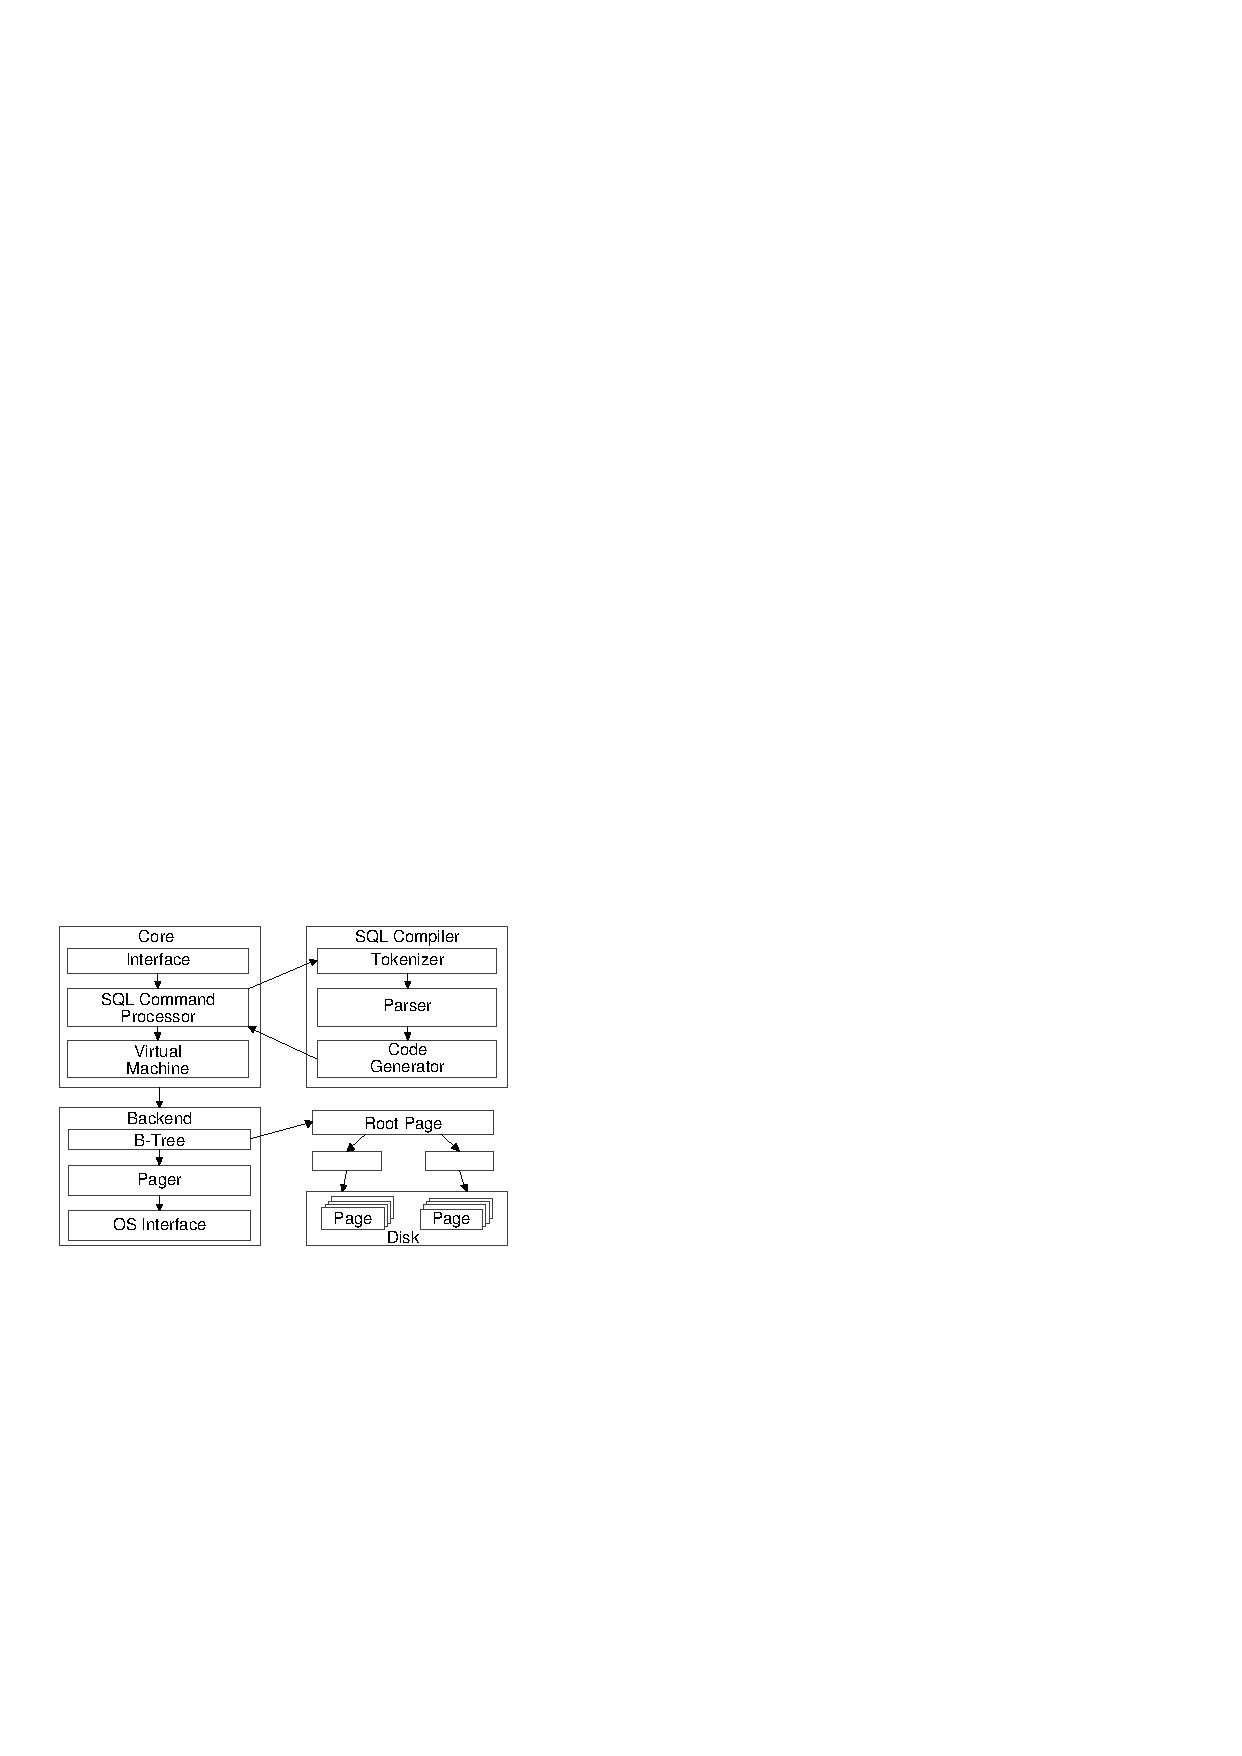
\includegraphics[width=0.5\textwidth]{pic/SQLite.pdf}
		\caption{Architecture of SQLite.}
		\label{fig:SQLite}
	\end{centering}
\end{figure}
SQLite is an in-process library, as well as an embedded SQL database widely used in mobile devices. Figure~\ref{fig:SQLite} gives the architecture of SQLite. SQLite exposes SQL interfaces to applications, and works by compiling SQL statement to bytecode, then running that bytecode using a virtual machine. When compiling one SQL statement, the SQL command processor first send it to the tokenizer. Then Tokenizer breaks the SQL statement into tokens and hands those tokens one by one to the parser. The parser assigns meaning to tokens based on their context, and assembles tokens into a pase tree. After this, the code generator runs to analyze the parser tree and generate bytecode that performs the work of the SQL statement.

The data organization of SQLite database is based B-tree. A separate B-tree is used for each table and index in the database. The B-tree module requests data from the disk in fixed-size pages. The pages can be either table B-tree page, index B-tree page, free page or overflow page. All pages are of the same size and are comprised of multi-byte fields. The pager is responsible for reading, writing, and caching these pages. SQLite communicates with the underlying file system by system
calls like {\tt open}, {\tt write} and {\tt fsync}. Also, SQLite use a journal mechanism for crush recovery, which makes database
file and journal file synchronized frequently with the disk and lead to a performance degradation consequently.


\section{LSM-tree-based Key-Value Database}
\begin{figure}[h]
	\centering
	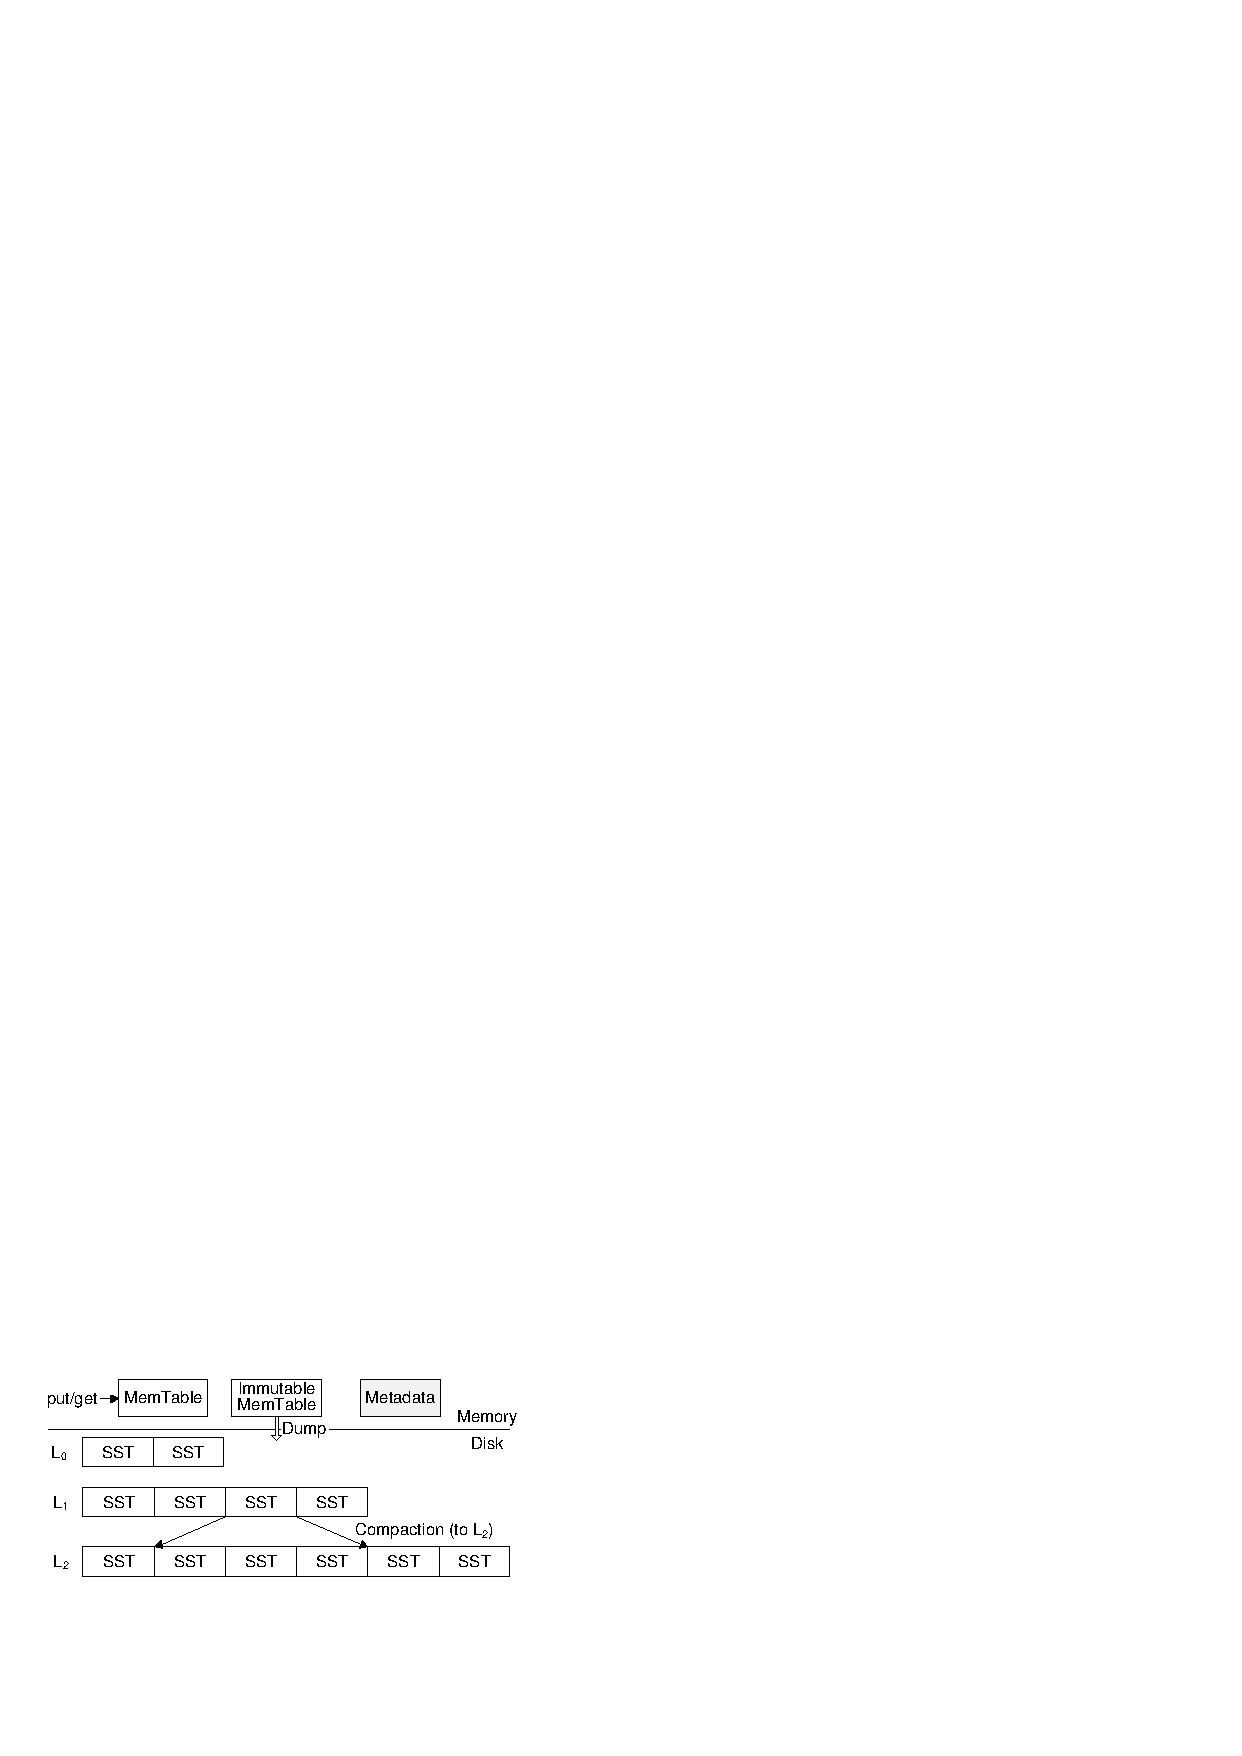
\includegraphics[width=0.5\textwidth]{pic/LSM-TREE.pdf}
	\caption{Architecture of LSM-tree-based Database.}
	\label{fig:LSM-TREE}
	\centering
\end{figure}
A LSM-tree-based key-value database maps a set of keys to the associated values. Applications access their data through simple {\tt SET} and {\tt GET} interfaces.
%We use an embedded LSM-tree-based key-value store SnappyDB~\cite{SnappyDB} to illustrate its working mechanism.
Figure~\ref{fig:LSM-TREE} describes the architecture of an LSM-tree-based key-value database implementation, which consists of two MemTables in main memory and a set of sorted string table (shown as SST in the figure) in the disk. To assist database query operations, meta-data, including indexes, bloom filters, key-value ranges and sizes of these in-disk SSTs are maintained in memory ~\cite{sears2012blsm}.

\begin{figure*}
	\centering
	\begin{minipage}[t]{0.4\textwidth}
		\centering
		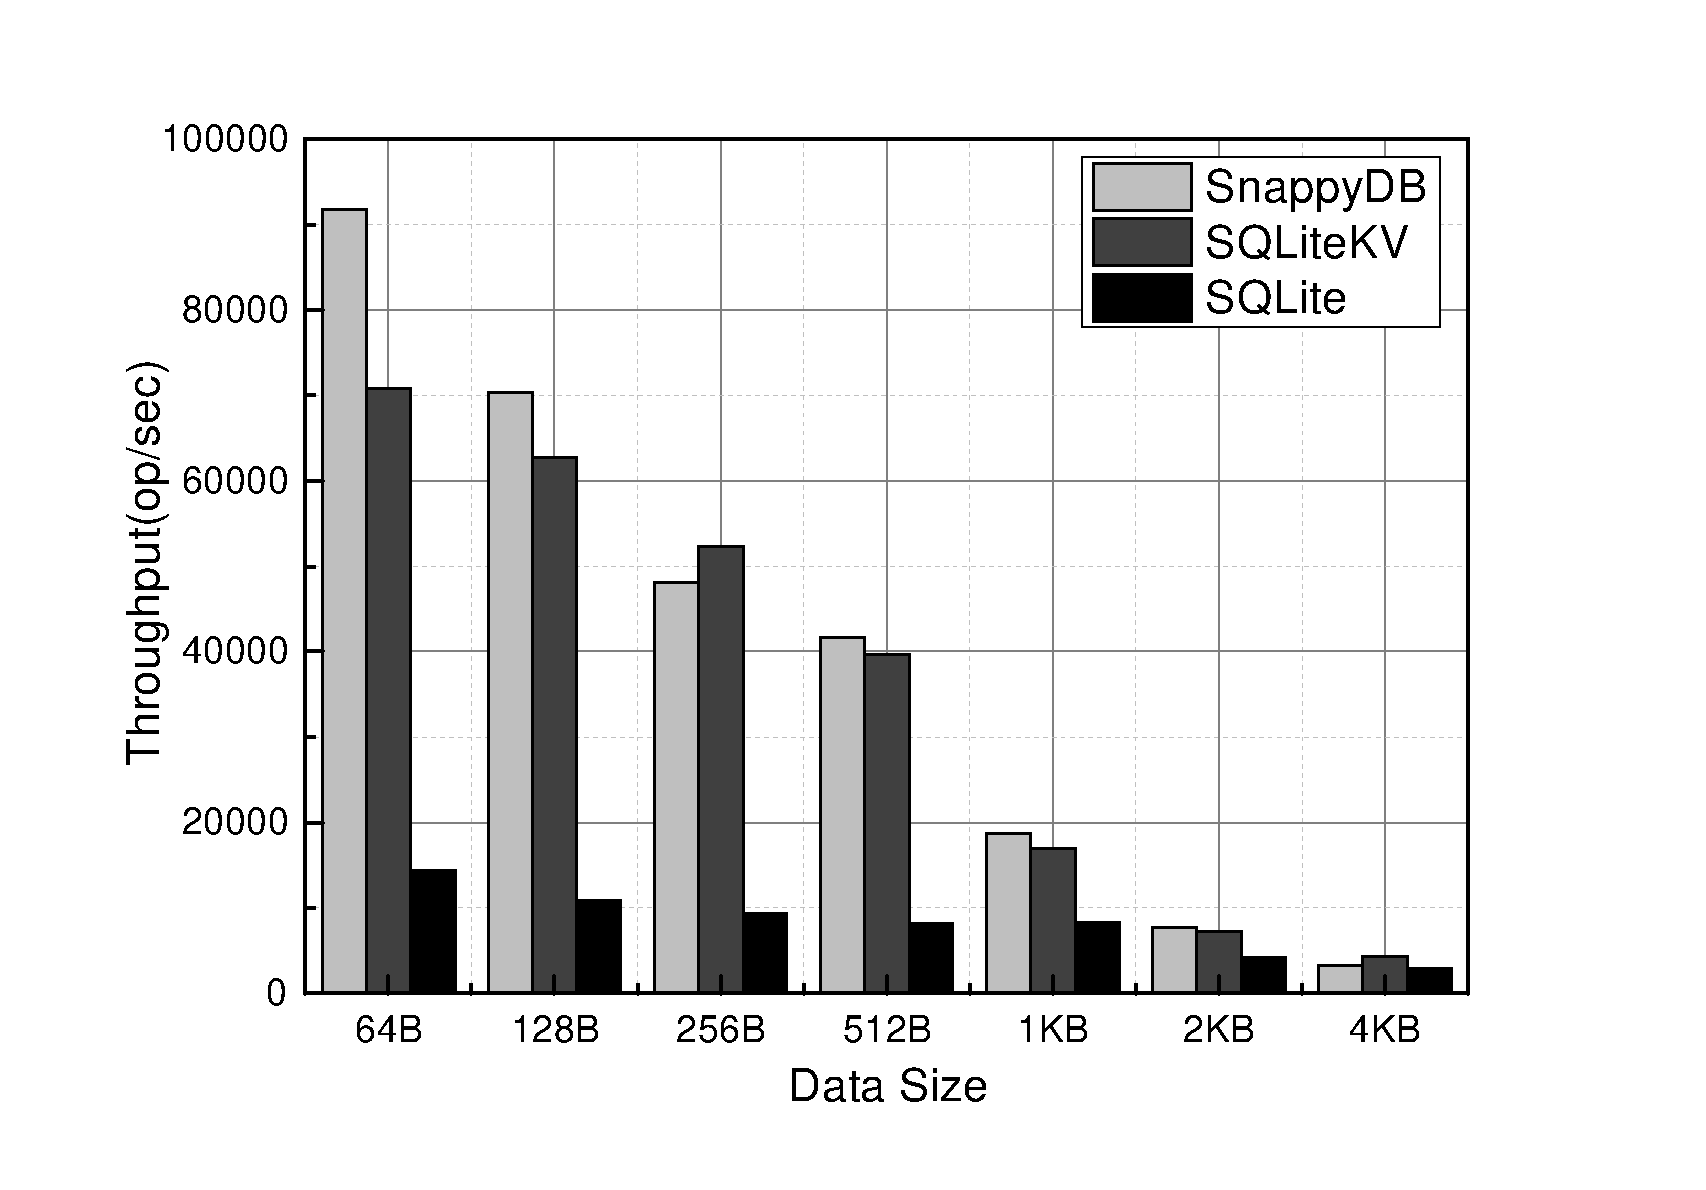
\includegraphics[width=0.95\textwidth]{Ext/workload1.pdf}
		\vspace*{-0.2cm}
		\caption{\small Throughput w. Insert operation.}
		\label{fig:mov_insert}
	\end{minipage}%
	\hspace*{0.7cm}
	\vspace{0.2cm}
	\begin{minipage}[t]{0.4\textwidth}
		\centering
		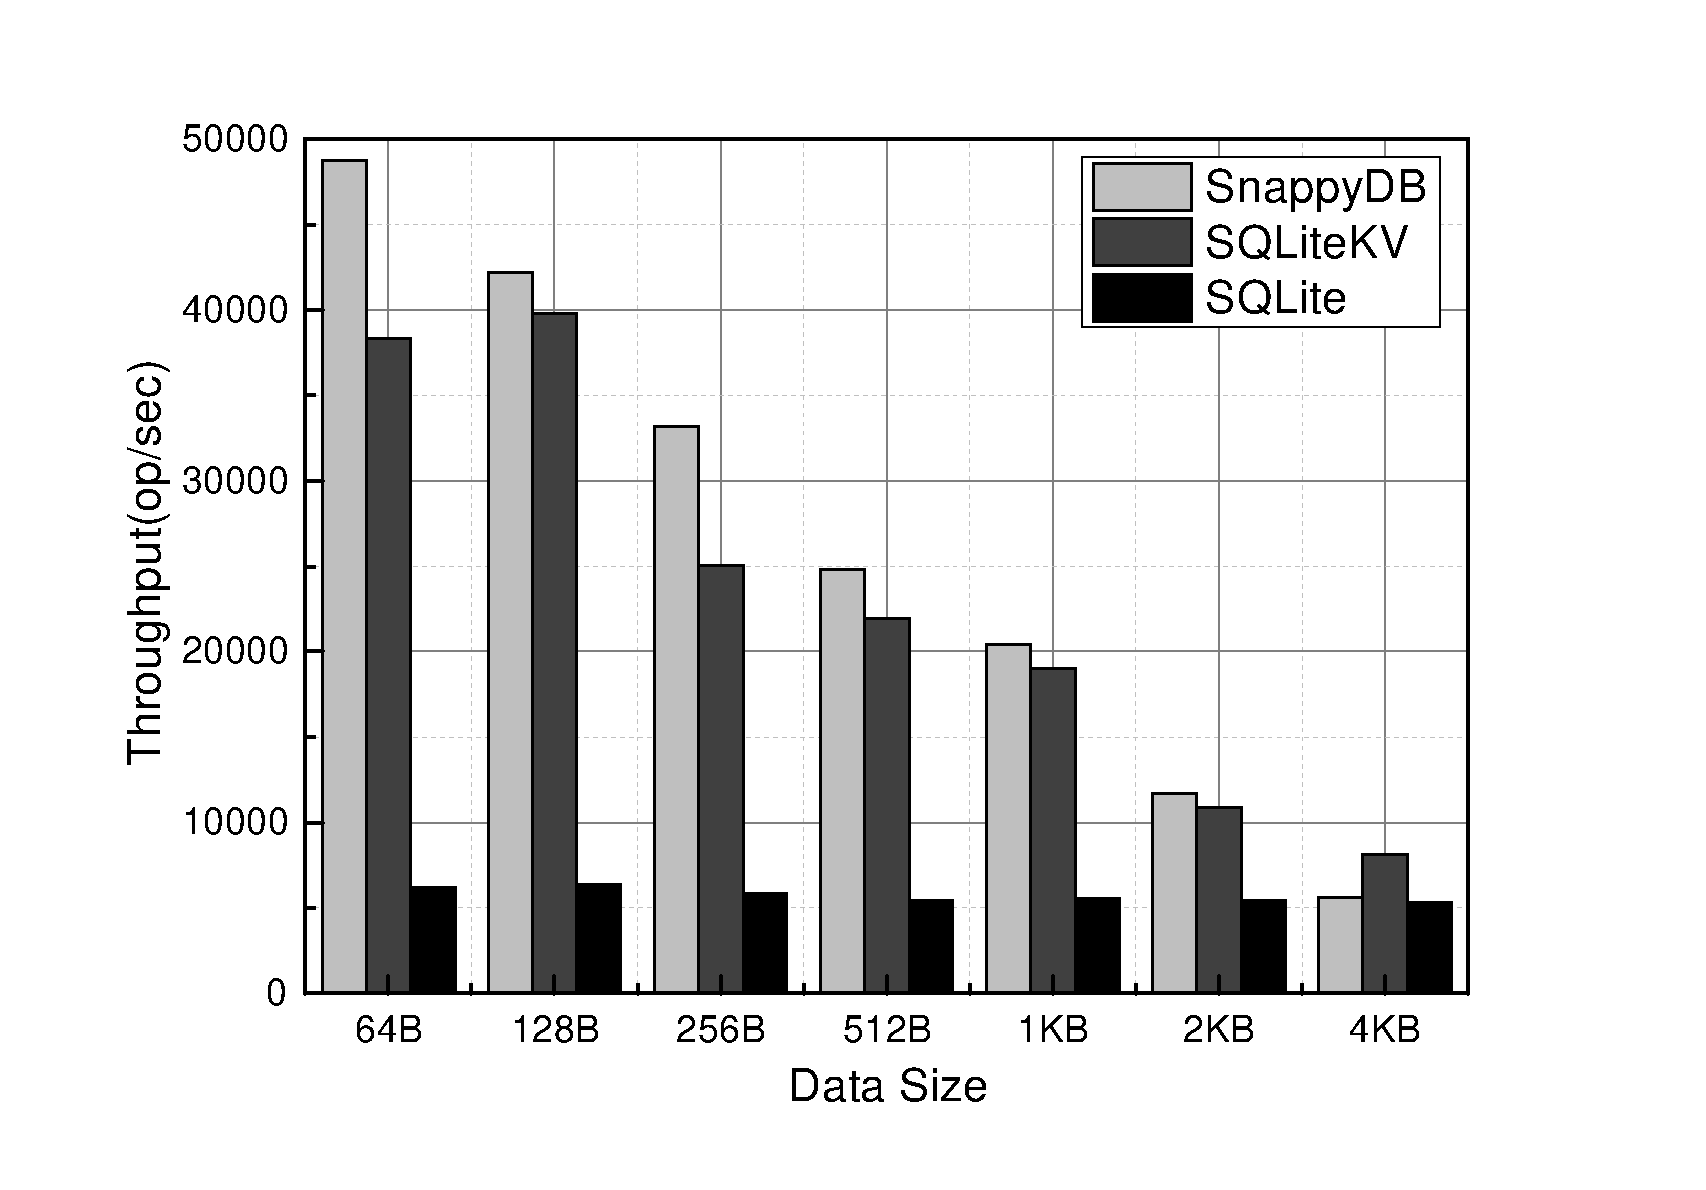
\includegraphics[width=0.95\textwidth]{Ext/workload2.pdf}
		\vspace*{-0.2cm}
		\caption{\small Throughput w. Query operation.}
		\label{fig:mov_query}
	\end{minipage}
	\vspace{0.2cm}
	\caption{\small Performance comparison of SQLite vs SnappyDB}
	\label{fig:motivation}
	\vspace*{-0.3cm}
\end{figure*}


The LSM-tree-based key-value design is based on two optimizations: (1) New data must be quickly admitted into the store to support high-throughput write. The database first use an in-memory buffer, called MemTable, to receive incoming key-value items. Once a MemTable is full, it is transferred into a sorted immutable MemTable, and dumped to disk SSTs. Key-value items in an SSTable are sorted according to their keys. Key range and a bloom filter of each SSTable that are maintained as metadata are cached in memory space to assist key-value search operations. (2) Key-value items in the store are sorted to support fast data location. A multilevel tree-like structure is build to progressively sort key-value items in this architecture. As shown in Figure~\ref{fig:LSM-TREE}, %new SSTables, which are just converted from immutable MemTables, are placed in Level0. 

The youngest level, \emph{Level 0}, is generated by writing the Immutable MemTable from memory to disk. Each level has a limit on the maximum number of SSTables. In order to keep the stored data in an optimized layout, a compaction process will be conducted to merge overlapping key-value items to the next level when the total size of \emph{Level L} exceeds its limit. 



\section{Other SQL-Compatible Key-Value Databases}
Apache Phoenix ~\cite{ApachePhoenix} is an open source SQL skin %relational database 
which receives SQL query by compiling it into a series of key-value operations of Apache HBase, a distributed, key-value, big data store. Phoenix provided a well-defined and industry standard APIs for OLTP and operational analytics for Hadoop. Nevertheless, without a deep integration with Hadoop framework, it is difficult for mobile devices to adopt either HBase as its storage engine or Phoenix for SQL-to-KV transitions. Besides, Phoenix, along with other Hadoop-related modules, is designed for scalable and distributed computing environments with large data sets ~\cite{forman1994challenges}, which means they can hardly fit in mobile environments as a matter of durability, battery life and portability ~\cite{sinha2016low}.

In this paper, we propose an efficient LSM-tree-based lightweight Database engine, SQLiteKV, which retains SQLite interface for mobile devices, keeps a high performance compared with SQLite and adopt an efficient LSM-tree structure on its storage engine.
